\documentclass[a4paper,table]{report}
\input{preamble_ask.tex}
\input{definitions_ask.tex}
\input{tikz.tex}
\input{myboxes.tex}

\geometry{left=1.9cm,right=1.9cm}
\input{insbox}
\pagestyle{askhseis}
\everymath{\displaystyle}
\usepackage{wrapfig}

\newcommand{\twocolumnsidescc}[2]{\begin{minipage}[c]{0.35\linewidth}\raggedright
        #1
        \end{minipage}\hfill\begin{minipage}[c]{0.60\linewidth}\raggedright
        #2
    \end{minipage}}
\newcommand{\twocolumnsidesccc}[2]{\begin{minipage}[c]{0.30\linewidth}\raggedright
        #1
        \end{minipage}\hfill\begin{minipage}[c]{0.67\linewidth}\raggedright
        #2
    \end{minipage}}
\newcommand{\twocolumnsidesccd}[2]{\begin{minipage}[c]{0.25\linewidth}\raggedright
        #1
        \end{minipage}\hfill\begin{minipage}[c]{0.67\linewidth}\raggedright
        #2
    \end{minipage}}

\begin{document}

\begin{center}
  \minibox{\large \bfseries \textcolor{Col1}{Προβλήματα Ακροτάτων}}
\end{center}

\vspace{\baselineskip}

\begin{mybox3}
\begin{problem}
  {\bfseries \boldmath Να προσδιοριστούν οι διαστάσεις μιας πισίνας 
    $ \SI{32}{m^3} $ με τετραγωνική βάση έτσι ώστε η επιφάνεια των εσωτερικών 
  τοίχων και του πυθμένα να είναι ελάχιστη.}
\end{problem}
\end{mybox3}
\begin{solution}
\item {}
  \InsertBoxR{2}{\parbox[b][\baselineskip][c]{0.30\textwidth}
    {\begin{tikzpicture}[scale=0.7]
        \node (0) at (0, 0) {};
        \node (1) at (3.5, 0) {};
        \node (2) at (5.5, 1) {};
        \node (3) at (2, 1) {};
        \node (4) at (0, 1.75) {};
        \node (5) at (3.5, 1.75) {};
        \node (6) at (5.5, 2.75) {};
        \node (7) at (2, 2.75) {};
        \draw (0.center) to node[below]{$x$} (1.center);
        \draw (1.center) to node[below]{$x$} (2.center);
        \draw[dashed] (2.center) to (3.center);
        \draw[dashed] (3.center) to (0.center);
        \draw (5.center) to (6.center);
        \draw (6.center) to (7.center);
        \draw (7.center) to (4.center);
        \draw (0.center) to (4.center);
        \draw (1.center) to node[below left,yshift=3pt]{$y$} (5.center);
        \draw (2.center) to (6.center);
        \draw[name path=a] (4.center) to (5.center);
        \path[name path=b] (3.center) to (7.center);
        \draw[dashed] [name intersections={of=a and b,by={x}}] (3.center) to (x) ;
        \draw [name intersections={of=a and b,by={x}}] (x.center) to (7.center) ;
  \end{tikzpicture}}}

  Το εμβαδό της πισίνας δίνεται από τη σχέση
  \inlineequation[eq:sur1]{E = x^{2} + 4xy}

  Ο όγκος της πισίνας είναι $V = 32 \Leftrightarrow  x^{2}y = 32$
  δηλαδή $\inlineequation[eq:vol1]{y = {32}/{x^{2}}}$.

  Άρα με αντικατάσταση της σχέσης~\eqref{eq:vol1} στη
  σχέση~\eqref{eq:sur1} έχουμε
  \begin{align*}
    E(x) = x^{2} + 4x\cdot \frac{32}{x^{2}} = x^{2} + \frac{128}{x}
  \end{align*}

  Αναζητάμε ελάχιστο για αυτή τη συνάρτηση.
  \begin{myitemize}
    \item $ E'(x) = 2x - \frac{128}{x^{2}} $ και $ E''(x) = 2 + \frac{256}{x^{3}} $
    \item $ E'(x) = 0 \Leftrightarrow 2x - \frac{128}{x^{2}} = 0
      \Leftrightarrow \frac{2x^{3} - 128}{x^{2}} = 0 \Leftrightarrow
      2x^{3} = 128 \Leftrightarrow x^{3} = 64 \Leftrightarrow$
      \inlineequation[eq:sta1]{\boxed{x = 4}}
    \item $ E''(4) = 2 + \frac{256}{64} = 6 > 0 $, επομένως πρόκειται για
      ολικό ελάχιστο.
  \end{myitemize}
  Με αντικατάσταση της σχέσης~\eqref{eq:sta1} στη σχέση~\eqref{eq:vol1} έχουμε 
  $ y = 2 $.

  Επομένως οι διαστάσεις της πισίνας πρέπει να είναι $ x = 4 $ και $ y = 2 $.
\end{solution}


\begin{mybox3}
\begin{problem}
  {\bfseries \boldmath Θεωρούμε τρίγωνο ΑΒΓ με  ΒΓ$=a $ και ύψος ΑΔ$=h$. Επίσης 
    θεωρούμε τα εγγεγραμένα σε αυτό ορθογώνια των οποίων η μία πλευρά βρίσκεται πάνω στη
  ΒΓ. Να βρεθεί εκείνο το παραλληλόγραμμο που έχει μέγιστο εμβαδό.}
\end{problem}
\end{mybox3}
\begin{solution}
  Το εμβαδό του ορθογωνίου δίνεται από τη σχέση $ E=xy $. Αρκεί να βρούμε μια σχέση που 
  να συνδέει τις πλευρές του ορθογωνίου $x$ και $y$ με τα γνωστά μεγέθη της άσκησης, 
  όπως είναι η πλευρά $a$ και το ύψος $h$ του τριγώνου. 
  Από την ομοιότητα των τριγώνων ΑΖΗ και ΑΒΓ, έχουμε ότι:

  \twocolumnsidescc{
    \begin{tikzpicture}[scale=0.85]
      \node (0) at (-2, 0) {};
      \node (1) at (3, 0) {};
      \node (2) at (-1, 2) {};
      \node (3) at (-1, 0) {};
      \node at (0) [left] {$B$};
      \node at (1) [right] {$\Gamma$};
      \node at (2) [above] {$A$};
      \node at (3) [below] {$\Delta$};
      \draw (0.center) to (1.center);
      \draw[name=ab] (0.center) to (2.center);
      \draw[name path=ac] (2.center) to (1.center);
      \draw[dashed] (2.center) -- (3.center)
        node[midway,right,yshift=-4pt] {$h$};
      \node at ($(0)!.65!(2)$) [left=3pt] {Z};
      \fill ($(0)!.65!(2)$) coordinate (z) circle[radius=1.5pt];
      \path[name path=zh] ($(0)!.65!(2)$) -- ([xshift=2pt]$(0)!.65!(2)$) 
        coordinate (f);
      \draw (z) -- (intersection of z--f and 2--1) coordinate (h);
      \node at (h) [right=8pt] {$H$};
      \fill (h) circle[radius=1.5pt];
      \draw (z) |- (3);
      \draw (h) |- (3);
      \fill (z|-3) coordinate (r) circle[radius=1.5pt];
      \fill (h|-3) coordinate (k) circle[radius=1.5pt];
      \fill (2|-z) coordinate (e) circle[radius=1.5pt];
      \node at (e) [above right,xshift=-1pt,yshift=-1pt] {$E$};
      \path (h)--(h|-3) node[midway,left]{y};
      \path (z|-3)--(h|-3) node[pos=.65,below]{x};
      \tkzMarkRightAngle(2,3,1);
  \end{tikzpicture}
  }{
  \[
    \frac{ZH}{B\Gamma} = \frac{AE}{A\Delta} \Leftrightarrow \frac{x}{a} = 
    \frac{h-y}{h} \Leftrightarrow x = \frac{a(h-y)}{h}
  \]
  Άρα, η σχέση για το εμβαδό, γίνεται:
  \[
    E(y) = \frac{a(h-y)}{h} y =  ay - \frac{a}{h} y^{2}
  \] 
}

Ζητάμε μέγιστο, οπότε έχουμε:
\begin{gather*}
  E'(y) = a - \frac{2a}{h} y \quad \text{και} \quad E''(y) = - \frac{2a}{h} \\
  E'(y)=0 \Leftrightarrow a - \frac{2a}{h} y = 0 \Leftrightarrow y= \frac{h}{2}
\end{gather*}
Για $ y=h/2 $ βρίσκουμε ότι $ x=a/2 $ και για να βεβαιώσουμε ότι πρόκειται για 
μέγιστο, έχουμε:
\[
  E''\left(\frac{h}{2}\right) = - \frac{2a}{h} < 0, \; \forall y \in \mathbb{R}
\] 
οπότε, το ορθογώνιο με διαστάσεις $ x=a/2 $ και $ y=h/2 $ έχει μέγιστο εμβαδό: 
$ E_{\max} = {ah}/{4}  $.
\end{solution}

\begin{mybox3}
\begin{problem}
  {\bfseries \boldmath Να εγγραφεί ορθογώνιο παραλληλόγραμμο με μέγιστο εμβαδό στην
  έλλειψη $ \frac{x^{2}}{a^{2}} + \frac{y^{2}}{b^{2}} = 1 $.} 
\end{problem}
\end{mybox3}
\begin{solution}
\item {}
  \twocolumnsidescc{
    \begin{tikzpicture}[shorten/.style={shorten >=#1pt,shorten <=#1pt},scale=0.8]
      \node (0) at (0, 2) {};
      \node (1) at (0, -2) {};
      \node (2) at (-3, 0) {};
      \node (3) at (3, 0) {};
      \node (6) at (-2, 0) {};
      \node (7) at (2, 0) {};
      \draw [bend right=90,thick] (6.center) edge [pos=.75] coordinate (l) (7.center);
      \fill (l) circle[radius=1.5pt];
      \draw [bend left=90,thick] (6.center) edge [pos=.75] coordinate (m) (7.center);
      \fill (m) circle[radius=1.5pt];
      \node at (m) [above right] {$M(x,y)$};
      \path [bend right=90] (7.center) edge [pos=.75] coordinate (k) (6.center);
      \fill (k) circle[radius=1.5pt];
      \path [bend left=90] (7.center) edge [pos=.75] coordinate (n) (6.center);
      \fill (n) circle[radius=1.5pt];
      \path (n) rectangle (m);
      \draw (n) rectangle (m);
      \path[name path=yy] (0.center) -- (1.center);
      \path[name path=xx] (2.center) -- (3.center);
      \draw (0.center) edge[latex-,thick] (1.center);
      \draw (2.center) edge[-latex,thick] (3.center);
      \path[name path=km] (k) -- (m);
      \path[name path=ml] (m) -- (l);
      \coordinate (o) (0,0);
      \coordinate[red,name intersections={of=km and yy,by=a}];
      \coordinate[red,name intersections={of=ml and xx,by=b}];
      \draw [decorate,shorten=0.5,decoration={brace,amplitude=3pt,raise=3pt}] (o) -- (a) 
        node[midway,left=6pt] {y} ; 
      \draw [decorate,decoration={brace,amplitude=3pt,raise=3pt}] (b) -- (o) 
        node[midway,below=6pt] {x} ; 
      \draw[fill,blue!20,draw=black] (0,0) rectangle (m);
      \node at (.7,.5) {$E_{1}$};
    \end{tikzpicture}
    }{
    Από το σχήμα, παρατηρούμε ότι λόγω συμμετρίας, θα έχουμε:
    \[
      E=4E_{1} \quad \text{όπου} \quad E_{1}=xy
    \] 
    Το σημείο $ M $ ανήκει στην έλλειψη, οπότε:
    \[
      \frac{x^{2}}{a^{2}} + \frac{y^{2}}{b^{2}} = 1 \overset{y>0}{\Leftrightarrow} y = 
      \frac{b}{a} \sqrt{a^{2}-x^{2}}
    \] 
  }

    Άρα το εμβαδό του ορθογωνίου, γίνεται:
    \[
      E_{1}=x  \frac{b}{a} \sqrt{ a^{2}-x^{2}} = \frac{b}{a} \sqrt{a^{2}x^{2}-x^{4}}
    \]
  Ζητάμε μέγιστο. Παρατηρούμε ότι 
  \[ 
    E_{1} \max \Leftrightarrow
    \frac{b}{a} \sqrt{a^{2}x^{2}-x^{4}} \max \overset{a,b>0}{\Leftrightarrow}
    \sqrt{a^{2}x^{2}=x^{4}} \max
    \overset{\sqrt{\cdot}\raisebox{1pt}{$\nearrow$}}{\Leftrightarrow} 
    f(x)=a^{2}x^{2}-x^{4} \max 
  \] 
  οπότε αρκεί να βρούμε μέγιστο για τη συνάρτηση $ f(x) $.
  \begin{gather*}
    f'(x)=2a^{2}x-4x^{3} \quad \text{και} \quad f''(x)=2a^{2}-12x^{2} \\
    f'(x)=0 \Leftrightarrow 2a^{2}x-4x^{3}=0 \Leftrightarrow 2x(a^{2}-2x^{2})=0
    \Leftrightarrow x = 0 \; \text{ή} \; x^{2}= a^{2}/2
  \end{gather*} 
  Η 1η λύση απορρίπτεται, οπότε $ x= \pm \frac{\sqrt{2}}{2} a \overset{x>0}{\Rightarrow}
  x = \frac{\sqrt{2}}{2} a $ και $ y= \frac{\sqrt{2}}{2} b $. Ελέγχουμε ότι πρόκειται 
  για μέγιστο.
  \[
    f''\left(\frac{\sqrt{2}}{2} a\right) = 2a^{2}-12 \frac{2a^{2}}{4} = - 4a^{2}<0
  \] 
  Επομένως το ορθογώνιο με πλευρές $ x= \frac{\sqrt{2}}{2} a $ και $ y =
  \frac{\sqrt{2}}{2} b $, έχει μέγιστο εμβαδό, $ E=4E_{1} = 2ab $.
\end{solution}

\begin{mybox3}
\begin{problem}
  {\bfseries \boldmath Ένα φύλλο ειδικού χαρτιού για μεγάλο μηχανολογικό σχέδιο, έχει
    επιφάνεια \SI{2}{m^{2}}. Στο σχέδιο που θα γίνει πρέπει να αφεθούν
    περιθώρια στην πάνω και στην κάτω πλευρά του σχεδίου, \SI{21}{cm}, ενώ
    στις πλαϊνές πλευρές \SI{14}{cm}. Ποιες πρέπει να είναι οι διαστάσεις
  τούτου φύλλου ώστε το καθαρό εμβαδό για σχεδίαση να είναι μέγιστο?}
\end{problem}
\end{mybox3}
\begin{solution}
\item {}
  \twocolumnsidesccc{
    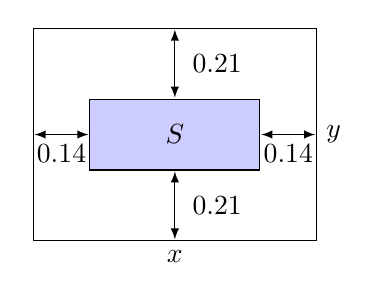
\begin{tikzpicture}[scale=0.9]
      \draw (0,0) rectangle (4,3);
      \draw[fill,blue!20] (.8,1) rectangle (3.2,2);
      \draw (.8,1) rectangle (3.2,2);

      \node at (2,1.5)  {$S$};
      \node at (2,0) [below] {$x$};
      \node at (4,1.5) [right] {$y$};
      \node (d) at (2,0.5) [right=.1cm] {\smaller$0.21$};
      \coordinate (dk) at (2,0) ;
      \coordinate (du) at (2,1) ;
      \node (p) at (2,2.5) [right=.1cm] {\smaller$0.21$};
      \coordinate (pk) at (2,2.0) ;
      \coordinate (pu) at (2,3) ;
      \draw (pk) edge[latex-latex,shorten >=0.5pt,shorten <=0.5pt,thin] (pu);
      \draw (dk) edge[latex-latex,shorten >=0.5pt,shorten <=0.5pt,thin] (du);
      \node (r) at (3.6,1.5) [below] {\smaller$0.14$};
      \coordinate (rl) at (3.2,1.5) ;
      \coordinate (rr) at (4,1.5) ;
      \draw (rl) edge[latex-latex,shorten >=0.5pt,shorten <=0.5pt,thin] (rr);
      \node (l) at (0.4,1.5) [below] {\smaller$0.14$};
      \coordinate (ll) at (0,1.5) ;
      \coordinate (lr) at (0.8,1.5) ;
      \draw (ll) edge[latex-latex,shorten >=0.5pt,shorten <=0.5pt,thin] (lr);
    \end{tikzpicture}
    }{
    Η επιφάνεια του χαρτιού είναι \SI{2}{m^{2}}, άρα $ E=2 \Leftrightarrow xy = 2
    \Leftrightarrow y= 2/x $. Σύμφωνα με το σχήμα το εμβαδό της περιοχής $S$ του 
    χαρτιού θα είναι:
    \[
      S = (x-2\cdot 0.14)(y-2\cdot 0.21) = (x-0.28)( \frac{2}{x} -0.42) = 2 -
      \frac{0.56}{x} - 0.42x+0.1176 
    \]
    Ζητάμε μέγιστο.
  } 

    \begin{gather*}
      S'(x)= \frac{0.56}{x^2} - 0.42 \quad\text{και}\quad S''(x)=-\frac{0.56}{x^{3}}
      \\
      S'(x)=0 \Leftrightarrow \frac{0.56}{x^{2}} -0.42 =0 \Leftrightarrow x^{2}=
      \frac{0.56}{0.42} \overset{x>0}{\Rightarrow} x= \sqrt{\frac{0.08}{0.06}}
      \Leftrightarrow x= \sqrt{\frac{4}{3}} = \frac{2 \sqrt{3}}{3} \quad \text{και} 
    \quad  y= \frac{2}{\sqrt{\frac{4}{3}}} = \sqrt{3}
    \end{gather*}
    Ελέγχουμε ότι πρόκειται για μέγιστο, οπότε
    \[
      S''\Big(\frac{2 \sqrt{3}}{3}\Big) = - 
      \frac{0.56}{\left(\frac{2 \sqrt{3}}{3} \right)^{2}} <0 
    \] 
    Επομένως η ορθογώνια περιοχή $S$ με διαστάσεις $ x= \frac{2 \sqrt{3}}{3} $ και 
    $ y= \sqrt{3} $ έχει μέγιστο εμβαδό.
\end{solution}

\begin{mybox3}
\begin{problem}
  {\bfseries\boldmath Δυο πόλεις Α και Β βρίσκονται προς το ίδιο μέρος της όχθης ενός
		ποταμού και απέχουν από αυτήν 10 και 15 χιλιόμετρα αντίστοιχα. Οι
		κάθετες προβολές των δύο πόλεων στην όχθη απέχουν 20 χιλιόμετρα. Οι δύο
		πόλεις πρέπει να εφοδιαστούν με νερό από ένα εργοστάσιο που θα
		κατασκευαστεί στην όχθη του ποταμού. Σε ποιο σημείο της όχθης πρέπει να
		κατασκευαστεί το εργοστάσιο ώστε για τους αγωγούς που θα συνδέσουν αυτό
  με τις πόλεις να έχουμε το ελάχιστο κόστος?}
\end{problem}
\end{mybox3}
\begin{solution}
\item {}
  \twocolumnsidescc{
    \begin{tikzpicture}[scale=0.8]
      \draw (-2,0) -- (5,0);
      \coordinate (a') at (-1,0) ;
      \coordinate (e) at (1,0) ;
      \coordinate (b') at (4,0) ;
      \coordinate (a) at (-1,2) ;
      \coordinate (b) at (4,3) ;
      \node (x) at (0,0) [below] {$x$};
      \node (x') at (2.5,0) [below] {$20-x$};
      \node at (a') [below] {$A'$} ;
      \node at (b') [below] {$B'$} ;
      \node at (e) [below] {$E$} ;
      \draw (a') edge[-] node[midway,left] {10} (a);
      \draw (b') edge[-] node[midway,right] {15} (b);
      \draw (a) edge[dashed] (e);
      \draw (b) edge[dashed] (e);
      \node at (a) [above] {$A$} ;
      \node at (b) [above] {$B$} ;
    \end{tikzpicture}
    }{
    Η απόσταση που συνδέει τις δύο πόλεις με το εργοστάσιο, θα είναι $ S=AE+BE $.
    \begin{align*}
      (AE)^{2}&=10^{2}+x^{2} \Rightarrow (AE)= \sqrt{100+x^{2}} \\
      (BE)^{2}&=15^{2}+(20-x)^{2} \Rightarrow (BE)= \sqrt{225+(20-x)^{2}} 
    \end{align*} 
    Άρα $ S(x) = (AE)+(BE) = \sqrt{100+x^2} + \sqrt{225 +(20-x)^{2}} $
  }

  Ζητάμε ελάχιστο
  \begin{gather*}
    S'(x) =  \frac{2x}{2 \sqrt{100+x^2}} + \frac{2(20-x)(-1)}{2 \sqrt{225+(20-x)^2}} \\
    S'(x)=0 \Leftrightarrow \frac{x}{\sqrt{100+x^2}} = \frac{20-x}{\sqrt{225+(20-x)^{2}}} 
    \Leftrightarrow \sqrt{\frac{225+(20-x)^{2}}{100+x^2}} = \frac{20-x}{x} 
    \Leftrightarrow \frac{225+(20-x)^{2}}{100+x^2} = \frac{(20-x)^2}{x^2} \\
    225x^2+\cancel{(20-x)^{2} x^{2}} = 100(20-x)^2+\cancel{x^{2}(20-x)^2} 
    \Leftrightarrow  \\ 
  \end{gather*} 
  \[
    \left.
      \begin{matrix}
        15x=10(20-x) \\
        15x=-10(20-x) 
      \end{matrix} \Leftrightarrow 
    \right\} \Leftrightarrow 
    \left.
      \begin{matrix}
        15x=200-10x \\
        15x=-200+10x 
      \end{matrix} 
    \right\} \Leftrightarrow 
    \left.
      \begin{matrix}
        25x=200 \\
        5x=-200 
      \end{matrix} 
    \right\} \Leftrightarrow 
    \left.
      \begin{matrix}
        x=8 \\
        x<0 \;\text{απορ.} 
      \end{matrix} 
    \right\}
  \]
  Ελέγχουμε ότι πρόκειται για ελάχιστο, οπότε
  \begin{align*}
    S''(x) &= \frac{\sqrt{100+x^2} -x \cdot \frac{2x}{x \sqrt{100+x^2}}}{(100+x^2)} +
    \frac{\sqrt{225+(20-x)^2} + (20-x)\cdot \frac{2(20-x)(-1)}{2
    \sqrt{225+(20-x)^2}}}{(225+(20-x)^2)^2} \\
           &= \frac{(100+x^2)-x^2}{\sqrt{100+x^2} \cdot (100+x^2)} +
    \frac{225+(20-x)^{2}-(20-x)^2}{\sqrt{225+(20-x)^2} \cdot (225+(x-20)^2)^2} \\
           &= \frac{100}{(100+x^2)^{3/2}} + \frac{225}{(225+(20-x)^2)^{3/2}} > 0, \;
           \forall x \in \mathbb{R} 
  \end{align*}
  άρα ελάχιστο.
\end{solution}

\begin{mybox3}
\begin{problem}
 {\bfseries\boldmath Να εγγραφεί σε κύκλο διαμέτρου $d$, ορθογώνιο με βάση $b$ και ύψος 
   $h$ ώστε το γινόμενο $ b h^{2} $ να είναι μέγιστο.}
\end{problem}
\end{mybox3}
\begin{solution}
\item {}
  \twocolumnsidesccd{
    \begin{tikzpicture}[scale=0.6]
      \draw[very thick,name path=circ] (0,0) circle (3cm) ;
      \path[name path=rect] (-3.5,-1.5) rectangle (3.5,1.5) ;
      \fill [name intersections={of=rect and circ,name=tom}] (tom-1) circle (1pt);
      \fill (tom-2) circle (1pt) ;
      \fill (tom-3) circle (1pt) ;
      \fill (tom-4) circle (1pt) ;
      \draw[thick,Col1] (tom-1) -- (tom-2) -- (tom-3) -- (tom-4) -- cycle ;
      \draw[thin,decorate,decoration={brace,amplitude=5pt,raise=4pt}] 
        ([xshift=3pt]tom-3) -- ([xshift=-3pt]tom-4) node[midway,above=8pt] {$b$} ;
      \draw[thin,decorate,decoration={brace,amplitude=5pt,raise=4pt}] 
        ([yshift=-3pt]tom-2) -- ([yshift=3pt]tom-3) node[midway,right=8pt] {$h$} ;
      \draw[dashed] (tom-3) -- coordinate[midway] (c) node [pos=0.6,above] {d} (tom-1) ;
      \fill (c) node[above left] {O} circle (2pt) ;
    \end{tikzpicture}
    }{
    Από το πυθαγόρειο θεώρημα έχουμε ότι $ d^{2}=b^{2}+h^{2} \Rightarrow
    h^{2}=d^{2}-b^{2} $ οπότε η ποσότητα $ bh^{2} $ γίνεται $ bh^{2}=b(d^{2}-b^{2}) =
    d^{2}b-b^{3} $. Άρα ζητάμε μέγιστο για τη συνάρτηση $ f(b) = d^{2}b-b^{3} $.
    \begin{gather*}
      f'(b) = d^{2}-3b^{2} \quad \text{και} \quad f''(b)=-6b \\
      f'(b)=0 \Leftrightarrow d^{2}-3b^{2}=0 \Leftrightarrow  b^{2} = \frac{d^{2}}{3}
      \overset{b>0}{\Rightarrow} b= \frac{\sqrt{3}}{3} d 
    \end{gather*}
    Τότε $ h^{2} = d^{2}- \frac{d^{2}}{3} = \frac{2d^{2}}{3}
    \overset{h>0}{\Rightarrow} h = \sqrt{\frac{2}{3}} d $.
  }

    Ελέγχουμε ότι πρόκειται για μέγιστο.
    $ f''\left(\frac{\sqrt{3}}{3} d\right) = -6 \frac{\sqrt{3}}{3} d = 
    -2 \sqrt{3} d < 0 $, άρα μέγιστο.
\end{solution}

\begin{mybox3}
\begin{problem} 
 {\bfseries\boldmath Να προσδιοριστεί ο λόγος της ακτίνας προς το ύψος ενός κλειστού
  κυκλικού ορθού κυλινδρικού δοχείου χωρητικότητας $c$ μονάδων όγκου, αν
  θέλουμε η επιφάνεια του δοχείου να είναι ελάχιστη.}
\end{problem}
\end{mybox3}
\begin{solution}
\item {}
  \twocolumnsidesccd{
    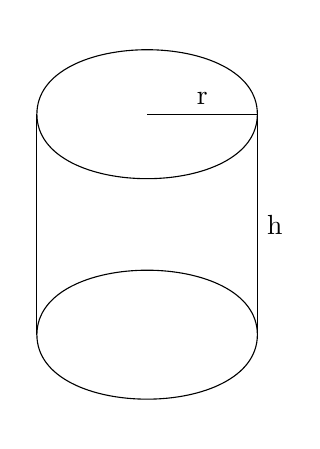
\begin{tikzpicture}[scale=0.7]
      \node (0) at (-2, 0) {};
      \node (1) at (2, 0) {};
      \node (2) at (-2, 0) {};
      \node (3) at (2, 0) {};
      \node (4) at (-2, 4) {};
      \node (5) at (2, 4) {};
      \node (6) at (-2, 4) {};
      \node (7) at (2, 4) {};
      \node (8) at (-2, 4) {};
      \node (9) at (2, 4) {};
      \node (10) at (-2, 4) {};
      \node (11) at (2, 4) {};
      \node (12) at (0, 4) {};
      \draw (2.center) to [bend right=90] (3.center);
      \draw (3.center) to [bend right=90] (2.center);
      \draw (10.center) to [bend left=90] (11.center);
      \draw (11.center) to [bend left=90] (10.center);
      \draw (11.center) to node[midway,right] {h} (3.center);
      \draw (10.center) to (2.center);
      \draw (12.center) to node[midway,above] {r} (11.center);
    \end{tikzpicture}
    }{
    Ο όγκος του δοχείου είναι $ V= \pi r^{2}h \Leftrightarrow c = \pi r^{2}h
    \Leftrightarrow h = \frac{c}{\pi r^{2}} $. 

    Το εμβαδό του δοχείου είναι $ S=2 \pi r^{2}+2 \pi r h = 2 \pi r^{2} + 
    2 \pi r \frac{c}{\pi r^{2}}$ 

    Επομένως $ S(r) = 2 \pi r^2 + \frac{2c}{r} $. Ζητάμε ελάχιστο.
    \begin{gather*}
      S'(r) = 4 \pi r - \frac{2c}{r^2} \quad \text{και} \quad S''(r) = 4 \pi +
      \frac{4c}{r^{3}} \\
      S'(r)=0 \Leftrightarrow 4 \pi r - \frac{2c}{r^{2}} = 0 \Leftrightarrow 4 \pi r^{3} =
      2c \Leftrightarrow r^{3} = \frac{c}{2 \pi} \Leftrightarrow r =
      \sqrt[3]{\frac{c}{2} \pi}
    \end{gather*}
  }
  Βρίσκουμε και το $h$. Έχουμε $ h = \frac{c}{\pi \cdot (\frac{c}{2 \pi} )^{2/3}} =
  \frac{2^{2/3} \cdot \pi ^{2/3} c}{\pi \cdot c^{2/3}} = 
  \frac{4^{1/3} c^{1/3}}{\pi ^{1/3}} = \left(\frac{4c}{\pi} \right)^{1/3} $  

  Ελέγχουμε ότι πρόκειται για μέγιστο.
  \[
    S''\left(\Bigl(\frac{c}{2 \pi} \Bigr)^{1/3}\right) = 4 \pi + \frac{4c}{\frac{c}{2 \pi}} = 12 \pi >0
  \] 
  Τελικά ο λόγος $ \frac{r}{h} $ θα είναι 
  \[ \frac{r}{h} = \frac{(\frac{c}{2 \pi})^{1/3} }{(\frac{4c}{\pi} )^{1/3}}
  = \frac{1}{2} \].
\end{solution}





\end{document}
